\section{Calculus}\label{sec:calculus}

In this section, we define a calculus that formally describes the operational semantics
of speculative nondeterminism. We first present the data models of the framework which
is independent of the rest of the calculus. Then we introduce the syntax of the language,
its typing and evaluation rules, and finally we discuss the exit and commit semantics
which are most interesting aspects of the framework.

\subsection{Data Model}\label{sec:datamodel}

In speculative nondeterminism, we assume a 
centralized data store acting as the primary programming environment. The implementation of this store is
not part of the language and therefore independent from the operational semantics of the language.
Here we present the abstract data model of the store that can be instantiated into different
concrete models.

A data model is a 6-tuple
$$\dm=\langle D_0,\alltype,\allop,\allstore,\vdash,\psi\rangle$$
where
\begin{description}
  \item[$D_0$] defines an empty data store, for example, 
    an empty set $\emptyset=\{\}$ or an empty multi-set $\lbb\rbb$.
  \item[$\alltype$] is the set of all possible data items in the data model.
    For example, $\alltype=\nat$ for data models such as a set of natural numbers. 
  \item[$\allop$] is the set of all data operations available in the data model.
  \item[$\allstore$] is the set of all possible data stores.
    For example, $\allstore=2^\nat$ for data models such as a set of natural numbers.
  \item[$\vdash\subseteq\allstore\times\allop$] is a binary relation denoted by $D\vdash d$.
    It defines when operation $d$ can be executed on the data store $D$.
    For example, if the operation $d$ has a precondition, $D\vdash d$ is
    true if and only if the condition is true when evaluated on the data store $D$.
  \item[$\psi:\allop\times\allstore\to\alltype\times\allstore$] is the transition function that
    defines the effect of data operations on the store. 
    In general, a data operation can do read, update, or both. 
    For read purpose, a data item $t\in\alltype$ in the data store must be returned from $\psi$. 
\end{description}

Next we give some examples of concrete data models under the above framework.

\subsubsection*{Tuple Space}

The idea of tuple space comes from Linda \cite{Gelernter85:Linda}, where
a tuple space is a multi-set of tuples that can be accessed concurrently.
A tuple is an ordered collection of fields. 
Agents can post their data to the tuple space in the form of tuples, and 
retrieve tuples as data from the tuple space that match a certain pattern.
There are three major operations in the tuple space data model:
(i) $\In$ reads and removes a tuple from a tuple space;
(ii) $\Out$ produces a tuple, writing it into a tuple space;
(iii) $\Rd$ non-destructively reads a tuple space and gets a copy of a tuple. 
Both $\In$ and $\Rd$ are blocking while $\Out$ is non-blocking.
Formal definitions and operational semantics for
the $\In/\Out/\Rd$ operations \cite{Ciancarini95}
can be easily adapted to this framework.

\subsubsection*{Key-value Store}

{\em Key-value store} is a mapping from keys 
to values, e.g.
$[a\mapsto 3, b\mapsto 5]$ is a key-value store
where the key $a$ gets value $3$ and $b$ gets $5$.
Typical data operations include: (i) creating a new key-value pair,
(ii) updating an existing key with a new value,
(iii) getting a value according to a key, and
(iv) removing a key and its corresponding value.
Conditional guards can also be combined with these data operations,
e.g., $a>4\Rightarrow b\gets 2$ waits (blocks) until
the condition $a>4$ is true in the store,
and then updates the value of $b$ to $2$.

\subsubsection*{Other Models}

Other more structured data models include relational data and logic programs.
Data operations are insertion and deletion of tuples/predicates. Applications
using these models are also typical.


\subsection{Syntax, Typing and Basic Operations}\label{sec:rules}

\begin{figure}
  \centering
  \begin{eqnarray*}
    a & ::= & [e,f] \text{ where } f:\allstore\to\nat \\
    e & ::= & e_1 \oplus e_2 \\ 
      &   | & e_1 . e_2 \\
      &   | & p \text{ where } p\in\allop \\
      &   | & \cm  ~~|~~ \cu  ~~|~~ \epsilon \\
      &     & \\
    U & ::= & \emptyset \\
      &   | & \{G_1,\dots,G_n\} \\
    G & ::= & \langle A,d,s \rangle \text{ where } d\in\allstore, s\in2^{\nat\times\nat} \\
      &   | & G_1 \oplus_k G_2 \text{ where $k\in\nat$ is the identifier of an agent} \\
    A & ::= & [] \\
      &   | & [a_1,\dots,a_m]
  \end{eqnarray*}
  \caption{Syntax and Runtime Data Structures}
  \label{fig:syntax}
\end{figure}

\figref{fig:syntax} first gives the syntax of agent programs 
for a data model.
\begin{description}
\item[$a$] is an agent $[e,f]$ where $e$ is the program and
	$f$ is the exit condition function.
\item[$e_1\oplus e_2$] is the exclusive choice construct.
\item[$e_1.e_2$] is the execution of $e_1$ and $e_2$ in a sequence.
\item[$p\in\allop$] is the data operation defined in the data model.
\item[$\epsilon$] is an empty program indicating the end of a program.
\item[$\cm$ and $\cu$] are primitives for pruning choices, which are described briefly in Section \ref{sec:overview} and formally in Section \ref{sec:commit2}. A well-formed program must have a matching $\cm$ for each choice construct.
However, our semantics framework can both add missing $\cm$'s and ignore redundant $\cm$'s automatically.
\end{description}

\figref{fig:syntax} also defines the runtime data structures 
in the calculus.
\begin{description}
\item[$U$] is a universe, the the top-level structure consisting of a set of galaxies.
The initial state of the universe is $\emptyset$.
\item[$G$] is the galaxy which is either a tree of worlds, or just one world.
A world is a quadruple $\langle A, d, s\rangle$ where $A$
is the list of agents participating in this world,
$d$ is the associated data store,
%$c$ is the set of indices (i.e., numeric identifiers) of committed agents,
and $s$ is the map from agent index to the exit value.
\end{description}

For simplicity we use numeric identifiers for agents throughout this paper.
We also use the following notations for the operations of a list:
(i) $|A|$ is the \emph{length} of the list $A$;
(ii) $A[\cdot]$ means \emph{indexing};
(iii) $A[i\mapsto a]$ replaces the $i$-th element of $A$ with $a$;
(iv) $A+B$ is the \emph{concatenation} of list $A$ and list $B$.

Top of \figref{fig:rules} shows the typing rules of the universe and galaxies.
$\typeof\cdot$ is a set of types which are defined in the given data model.
The set of types of the universe is the union of the sets of types of all the galaxies, 
while the set of types of a galaxy is the union of the sets of types of all the leaf worlds. 
Note that all the types come from the data model.

\begin{figure*}
\begin{minipage}{\textwidth}
  \flushright\fbox{$T=S$} \\
  \begin{minipage}{0.24\textwidth}
    \begin{gather*}
    \frac{}{\typeof U = \bigcup_{G\in U} \typeof G} \\
    \frac{
        {a=[e,f]}\qquad
        {\typeof e = \tau_1}}
      {\typeof a = \tau_1}
    \end{gather*}
  \end{minipage}
  \begin{minipage}{0.24\textwidth}
    \begin{gather*}
    \frac{
        {G = \langle A,d,s\rangle}\quad
        {\dstype(d) = \tau_1}}
    {\typeof{G} = \tau_1} \\
    \frac{
        {\typeof{e_1} = \tau_1}\qquad
        {\typeof{e_2} = \tau_2}}
    {\typeof{e_1\oplus e_2} = \tau_1\cup\tau_2}
    \end{gather*}
  \end{minipage}
  \begin{minipage}{0.24\textwidth}
    \begin{gather*}
    \frac{
        {\typeof{G_1} = \tau_1}\qquad
        {\typeof{G_2} = \tau_2}}
    {\typeof{G_1\oplus G_2} = \tau_1\cup\tau_2} \\
    \frac{
        {\typeof{e_1} = \tau_1}\qquad
        {\typeof{e_2} = \tau_2}}
    {\typeof{e_1.e_2} = \tau_1\cup\tau_2}
    \end{gather*}
  \end{minipage}
  \begin{minipage}{0.12\textwidth}
    \begin{gather*}
    \frac{p \in \allop}{\typeof{p} = \{\dptype(p)\}} \\
    \frac{\quad}{\typeof{\cm} = \emptyset}
    \end{gather*}
  \end{minipage}
  \begin{minipage}{0.12\textwidth}
    \begin{gather*}
    \frac{\quad}{\typeof{\epsilon} = \emptyset} \\
    \frac{\quad}{\typeof{\cu} = \emptyset}
    \end{gather*}
  \end{minipage}
  %%%%
  \flushright\fbox{$U+a\Longrightarrow U'$}
  \[
    \tag{\sc Entrance}\label{rule:birth}
    \frac{}{U + a \Longrightarrow U\cup\{\langle [a],\mkstore,\emptyset,\emptyset\rangle\}}
  \]
  \flushright\fbox{$U\uto U'$}
  \[
    \tag{\sc Merge}\label{rule:merge}
    \frac{
    {\begin{matrix}
              w=\langle A,d,s\rangle \\
              w'=\langle A[i\mapsto[e,f]],d',s'\rangle \\
              s'=\snapshot(s,|e|,i,f(d'))
            \end{matrix}}
            \qquad
    {\begin{matrix}
              G,G'\in U \\
              w\in leaves(G)
            \end{matrix}}
            \qquad
    {\begin{matrix}
              p\in\allop \\
              d\vdash p \\
              d'=\dtrans(p,d)
            \end{matrix}}
            \qquad
    {\begin{matrix}
              {\begin{matrix}
                [p.e,f] = A[i] \\
                \dptype(p)\in\typeof{G'}
              \end{matrix}}
              \qquad
              (1\le i\le |A|)
            \end{matrix}}}
    {U \uto (U\setminus\{G,G'\}) \cup \{\gmerge(replace(G,w,w'),G')\}}
  \]
  \[
    \tag{\sc Alone}\label{rule:alone}
    \frac{
    {\begin{matrix}
              w=\langle A,d,s\rangle \\
              w'=\langle A[i\mapsto[e,f]],d',s'\rangle \\
              s'=\snapshot(s,|e|,i,f(d'))
            \end{matrix}}
            \qquad
    {\begin{matrix}
              G\in U \\
              w\in leaves(G)
            \end{matrix}}
            \qquad
    {\begin{matrix}
              p\in\allop \\
              d\vdash p \\
              d'=\dtrans(p,d)
            \end{matrix}}
            \qquad
    {\begin{matrix}
              {\begin{matrix}
                [p.e,f] = A[i] \\
                \dptype(p)\not\in\typeof{U\setminus\{G\}}
              \end{matrix}}
              \qquad
              (1\le i\le |A|)
            \end{matrix}}}
    {U \uto (U\setminus\{G\}) \cup \{replace(G,w,w')\}}
  \]
%
  \flushright\fbox{$G\gto G'$}\\
  \begin{minipage}{0.59\textwidth}
  \[
    \tag{\sc Fork}\label{rule:fork}
    \frac{
    {[(e_1\oplus e_2).e,f]=A[i]}\qquad
%    {H=A[1..i-1]+A[i+1..|A|]}\quad
%    {c'=shiftc(c,i)}\quad
%    {s'=rs(s,i,|A|)}\quad
    {(1\le i\le |A|)}}
    {\langle A,d,s\rangle \gto
      \langle A[i\mapsto[e_1.e,f]],d,s\rangle \oplus_i
      \langle A[i\mapsto[e_2.e,f]],d,s\rangle}
  \]
  \[
    \tag{\sc Cm}\label{rule:cm}
    \frac{
    {[\cm.e,f]=A[i]}\qquad
%    {\{i+1,\dots,|A|\}\subseteq c}\qquad
    {(1\le i\le |A|)}}
    {G\oplus_i\langle A,d,s\rangle \gto \langle A[i\mapsto[e,f]],d,\snapshot(s,|e|,i,f(d))\rangle}
  \]
  \end{minipage}
  \begin{minipage}{0.4\textwidth}
  \[
    \tag{\sc Swap}\label{rule:swap}
    \frac{}{G_1\oplus_k G_2 \gto G_2\oplus_k G_1}
  \]
  \[
    \tag{\sc Cu}\label{rule:cu}
    \frac{
    {[\cu.e,f]=A[i]}\qquad
    {(1\le i\le |A|)}}
    {\langle A,d,s\rangle\oplus_k G \gto G}
  \]
  \end{minipage}
  \vspace{1ex}
  \[
    \tag{\sc Cm-Auto}\label{rule:cm-auto}
    \frac{
      w\in leaves(G) \qquad
      w=\langle A,d,s\rangle \qquad
      [\epsilon,f]=A[i] \qquad
      i\in cid(G) \qquad
      w'=\langle A[i\mapsto[\cm,f]],d,s\rangle \qquad
      (1\le i\le |A|)
    }
    {G \gto replace(G,w,w')}
  \]
  \[
    \tag{\sc Cm-Skip}\label{rule:cm-skip}
    \frac{
      w\in leaves(G) \qquad
      w=\langle A,d,s\rangle \qquad
      [\cm.e,f]=A[i] \qquad
      i\not\in cid(G) \qquad
      w'=\langle A[i\mapsto[e,f]],d,s\rangle \qquad
      (1\le i\le |A|)
    }
    {G \gto replace(G,w,w')}
  \]
  \vspace{1ex}
  \[
    \tag{\sc Exit}\label{rule:exit}
    \frac{%\displaystyle
    W=leaves(G)
    \qquad \sum_{w\in W} ins(w,i)=0
    \qquad i\not\in cid(G)
    \qquad \left|\bigcup_{w\in W} \{exitval(w,i)\}\right|=1
    \qquad (1\le i\le\max_{w\in W} |w|)}
    {G \gto remove(G,i)}
  \]
  \vspace{1mm}
\end{minipage}
%
\begin{minipage}{0.49\textwidth}\centering
  \begin{gather*}
%    \frac{c'=\{j\in c:j<i\}\cup\{j-1:j\in c \land j>i\}}{shiftc(c,i) = c'} \\
    \frac{s'=\{\langle j,v\rangle\in s:j<i\}\cup\{\langle j-1,v\rangle:\langle j,v\rangle\in s \land j>i\}}{shifts(s,i) = s'}
%    \frac{i\in c}{rc(c,i,m) = shiftc(c,i) \cup \{m\}} \qquad
%    \frac{i\not\in c}{rc(c,i,m) = shiftc(c,i)} \\
%    \frac{\langle i,v\rangle\in s}{rs(s,i,m) = shifts(s,i) \cup \{\langle m,v\rangle\}} ~
%    \frac{i\not\in\{j:\langle j,v\rangle\in s\}}{rs(s,i,m) = shifts(s,i)}
  \end{gather*}
  \begin{gather*}
    \frac{\langle G',r\rangle = rg(G,w,w')}
    {replace(G,w,w') = G'} \\
    \frac{\langle G_1',\textbf{true}\rangle = rg(G_1,w,w')}
    {rg(G_1\oplus_k G_2,w,w') = \langle G_1'\oplus_k G_2,\textbf{true}\rangle} \\
    \frac{\langle G_1',\textbf{false}\rangle = rg(G_1,w,w') \qquad \langle G_2',r\rangle = rg(G_2,w,w')}
    {rg(G_1\oplus_k G_2,w,w') = \langle G_1'\oplus_k G_2',r\rangle} \\
    \frac{}{rg(w,w,w') = \langle w',\textbf{true}\rangle} \qquad
    \frac{w_1\ne w}{rg(w_1,w,w') = \langle w_1,\textbf{false}\rangle}
  \end{gather*}
  \[
  % exitval
    %\tag{\sc EVal}
    \frac{w=\langle A,d,s\rangle \qquad \langle i,v\rangle\in s}
    {exitval(w,i)=v}
  \qquad
    \frac{w=\langle A,d,s\rangle}{|w|=|A|}
  \]
  \[
    \frac{}{\snapshot(s,0,i,v)=s\cup\{\langle i,v\rangle\}}
    \qquad
    \frac{l>0}{\snapshot(s,l,i,v)=s}
  \]
  \begin{gather*}
    \frac{}{|e_1\oplus e_2|=\max(|e_1|,|e_2|)}
    \qquad
    \frac{}{|e_1.e_2|=|e_1|+|e_2|}
  \\
    \frac{p\in\allop}{|p|=1}
    \qquad
    \frac{}{|\epsilon|=0}
    \qquad
    \frac{}{|\cm|=1}
    \qquad
    \frac{}{|\cu|=1}
  \end{gather*}
\end{minipage}
\hspace{5mm}
\begin{minipage}{0.49\textwidth}\centering
  %% galaxy merging functions
  \begin{gather*}
    \frac
      {G=G_1\oplus_k G_2}
      {\gmerge(G,G')=\gmerge(G_1,G')\oplus_k\gmerge(G_2,G')}
  \\
    \frac{}{\gmerge(w,G')=\gpaste(w,G')}
  \end{gather*}
  \begin{gather*}
    \frac
      {w=\langle A,d,s\rangle
      \qquad
      G=G_1\oplus_k G_2}
      {\gpaste(w,G)=\gpaste(w,G_1)\oplus_{k+|w|}\gpaste(w,G_2)}
  \\
    \frac
      {\begin{matrix}
        w=\langle A_0,d_0,s_0\rangle \qquad
        G=\langle A,d,s\rangle \\
        s'=s_0\cup\{\langle i+|w|,v\rangle:\langle i,v\rangle\in s\}
      \end{matrix}}
      {\gpaste(w,G)=\langle A_0+A,d_0\sqcup d,s'\rangle}
  \end{gather*}
  %%
  \[
    \frac{}{cid(G_1\oplus_k G_2)=cid(G_1)\cup cid(G_2)\cup\{k\}} \qquad
    \frac{}{cid(w)=\emptyset}
  \]
  %% Auxiliary Functions for Exit Inference Rules
  \[
  % leaves
    \frac{G=G_1\oplus_k G_2}{leaves(G)=leaves(G_1)\uplus leaves(G_2)}
    \quad
    \frac{}{leaves(w)=\lbb w\rbb}
  \]
  \[
  % #instr
    \frac{w=\langle A,d,s\rangle \qquad [e,f]=A[i] \qquad (1\le i\le |A|)}
    {ins(w,i)=|e|}
  \]
  \begin{gather*}
  % remove
    \frac{G=G_1\oplus_k G_2}
    {remove(G,i)=remove(G_1,i)\oplus_k remove(G_2,i)}
  \\
    \frac{\begin{matrix}
        w=\langle A,d,s\rangle \qquad
%        c'=shiftc(c,i) \qquad
        s'=shifts(s,i)
    \end{matrix}}
    {remove(w,i)=\langle A[1..i-1]+A[i+1..|A|],d,s'\rangle}
  \end{gather*}
\end{minipage}
%
  \caption{Inference Rules}
  \label{fig:rules}
\end{figure*}

\figref{fig:rules} shows all the inference rules used to implement our framework.
The system starts with an empty universe $\emptyset$.
New agents can dynamically enter the system via the $+$ operator.
The entrance of a new agent will create a galaxy with one world by itself,
as shown in \ref{rule:birth}.

When one of the agents is ready to execute some operation $p$
on the data store $d$ (i.e., $d\vdash p$),
rules \ref{rule:merge} and \ref{rule:alone} force the checking of
types involved in that operation.
As mentioned in Section \ref{sec:overview},
worlds are partitioned into galaxies according
to the interests of their associated agents at run-time.
The interest is, in fact, the types here.
\ref{rule:merge} shows the case when the type of the operation $p$
interleaves with the type of galaxy $G'$.
In this case, the current galaxy $G$, has to be merged with the galaxy $G'$,
which contains the required type.
In case there is no need to merge with other galaxies,
i.e., either the type resides in the current galaxy or it is a new type,
the operation $p$ is executed directly,
as shown in rule \ref{rule:alone}.

The main idea of speculative nondeterminism is forking and pruning of choices.
\ref{rule:fork} fires if an agent is reduced to
a choice $(e_1\oplus e_2) .e$,
and it consumes the choice construct in the agent to split the current world of
the agent into two.
When the agent on the lowest level of the galaxy tree structure
executes $\cm$, as shown in rule \ref{rule:cm},
the other side of the choice is pruned.
Similarly, for $\cu$ operations, the current side of the choice is pruned instead,
as shown in rule \ref{rule:cu}.
The key difference between $\cm$ and $\cu$ is that
$\cu$ can be executed in any agent and cause the pruning to takes place immediately,
while $\cm$ can only be executed in the lowest-level agents which are
more localized and less aggressive.
Also $\cm$ is blocking when it is not on the lowest level of the tree,
because non-blocking $\cm$ here potentially consumes more resources 
under the risk of being pruned by the $\cm$ on the lowest level. 
This form of commit semantics is therefore known as \emph{localized commit},
which is described in more details in Section \ref{sec:commit2}.
Finally, the rule \ref{rule:cm-auto} automatically adds a $\cm$ at the end of a program 
in case the program is ill-formed and doesn't have a commit operator that matches
a choice. 
Rule \ref{rule:cm-skip} handles another kind of ill-formed program where
there is more than one $\cm$ for a choice branch. 
In this case, only the first $\cm$ is honored but all subsequent ones are ignored.
We don't need a similar skip rule for $\cu$ because the first $\cu$ in a branch
already prunes the current branch.

Rules without names define the following auxiliary functions.
\begin{description}
\item[$shifts(s,i)$] removes the snapshot of $i$ (i.e. $\langle i,v\rangle$) from $s$ (if applicable) and shifts the indices by 1 of snapshots with index greater than $i$.
A \emph{snapshot} is a pair $\langle i,v\rangle$ where $i$ is an agent's index, and $v$ is the evaluation result of the exit condition function $f_i$ of the agent $i$ at the point of time when agent $i$ finishes execution.
\item[$replace(G,w,w')$] replaces world $w$ in galaxy $G$ with $w'$.
\item[$rg(G,w,w')$] is a helper function for $replace$.
\item[$\gmerge(G,G')$] merges 2 galaxies by pasting $G'$ to the leaves of $G$.
\item[$\gpaste(w,G)$] pastes the copies of $w$ to the leaves of $G$.
\item[$cid(G)$] is the set of all the choice identifiers in $G$.
\end{description}

The transitions on the universe and the galaxies have the following properties. 

\begin{proposition}
The data types of galaxies are disjoint.
\end{proposition}
\begin{proof}[Proof sketch]
For \ref{rule:birth}, $\forall G\in U, \typeof G \cap \typeof\mkstore = \emptyset$.
%
For \ref{rule:merge}, % $\dptype(p)\in\typeof{G'}$, and by the definition of data model,
$\typeof{w'}=\dstype(d')=\dstype(\dtrans(p,d))\subseteq\dstype(d)\cup\{\dptype(p)\}$
$\Rightarrow \typeof{w'}\subseteq\dstype(d)\cup\typeof{G'}=\typeof w\cup\typeof{G'}$. 
\begin{align*}
    & \typeof{\gmerge(replace(G,w,w'),G')} \\
  = & \typeof{replace(G,w,w')}\cup\typeof{G'} \\
  \subseteq & {\textstyle\left(\bigcup_{\tilde w \in leaves(G)\setminus\{w\}} \typeof{\tilde w}\right)} \cup \typeof w\cup\typeof{G'} \\
  = & \typeof G \cup \typeof{G'}
\end{align*}
\begin{align*}
  & \forall G_1\in U, \typeof{G_1}\cap\typeof G=\emptyset, \typeof{G_1}\cap\typeof{G'}=\emptyset  \\
  \Rightarrow & \typeof{G_1} \cap (\typeof{G}\cup\typeof{G'}) = \emptyset \\
  \Rightarrow & \typeof{G_1} \cap \typeof{\gmerge(replace(G,w,w'),G')} = \emptyset
\end{align*}
The same applies to \ref{rule:alone}. 

For rules \ref{rule:fork}, \ref{rule:swap}, \ref{rule:cm}, and \ref{rule:exit}, 
the data stores do not change. 
%
For \ref{rule:cu}, data store $d$ is removed. 
Let $G_0=\langle A,d,c,s\rangle\oplus G$.
\begin{align*}
  \forall G_1\in U, \typeof{G_1}\cap\typeof{G_0}=\emptyset
  & \Rightarrow \forall t\in\typeof{G_1}, t\not\in\typeof{G_0} \\
  \typeof{G_0}=\dstype(d)\cup\typeof G
%  & \Rightarrow t\not\in\dstype(d)\text{ and }t\not\in\typeof G \\
  & \Rightarrow t\not\in\typeof G \\
  & \Rightarrow \typeof{G_1}\cap\typeof G=\emptyset
\end{align*}
\end{proof}

\begin{proposition}
An agent lives in one and only one galaxy.
\end{proposition}
\begin{proof}[Proof sketch]
For \ref{rule:birth}, $a$ by itself is one galaxy.

For \ref{rule:merge}, assume $a$ lives in only one galaxy in $U$. 
If $a$ lives in $G$ or $G'$, it still lives in $\gmerge(replace(G,w,w'),G')$.
Otherwise, it lives in $U\setminus\{G,G'\}$.
The same applies to \ref{rule:alone}. 

All the other rules do not move agents between galaxies. 
\end{proof}

\begin{proposition}
Given the empty universe and $n$ agents each with at most $k$ choices, 
if $\bigcap_{i=1}^n \typeof{a_i} = \emptyset$ then the number of simultaneous worlds is at most $kn$.
\end{proposition}
\begin{proof}[Proof sketch]
$\bigcap_{i=1}^n \typeof{a_i} = \emptyset \Rightarrow \forall 1\le i<j\le n, \typeof{a_i}\cap\typeof{a_j}=\emptyset.$
So all the agents live in their own galaxies and will not merge together. 
Then there will be $n$ galaxies. 
For $k$ choices there will be at most $k$ worlds corresponding to them. 
Hence, the number of simultaneous worlds is at most $kn$.
\end{proof}


\subsection{Exit Semantics}\label{sec:exit}

Rule \ref{rule:exit} in Figure \ref{fig:rules} shows the exit semantics.
\begin{description}
\item[$leaves(G)$] returns a multi-set of the leaf worlds in the tree structure of a galaxy $G$.
\item[$ins(w,i)$] counts the number of instructions left (to be executed) in the $i$-th agent program in world $w$.
\item[$exitval(w,i)$] retrieves the evaluation result of the exit condition function of the $i$-th agent when it stops in world $w$.
\item[$|w|$] is the number of agents in world $w$.
\item[$remove(G,i)$] removes the $i$-th agents from all the worlds in galaxy $G$.
\end{description}

Basically \ref{rule:exit} lists all the worlds in the galaxy, counts the number of instructions to ensure the $i$-th agent has completed (i.e. reduced to the empty program $\epsilon$) in all the worlds, and applies the exit condition function to ensure the evaluated results are the same across all the worlds.
When all these conditions are satisfied, the $i$-th agent can exit from the galaxy.

In general, if the states are \emph{consistent} across all the worlds at
the point when the agent completes, the agent can exit immediately.
However, the agent may complete at different wall clock times in different worlds.
In order to capture the values of the exit condition function $f$ applied to different worlds,
$f$ has to be evaluated immediately when the agent becomes $\epsilon$ in a world,
and the evaluated results, namely \emph{snapshots}, are stored as meta data of that world.
The meta data  persists even if this world evolves into multiple worlds later.

Formally, for a world $\langle A,d,s\rangle$,
the snapshots are stored in the map $s$.
At the bottom of Figure \ref{fig:rules},
the function $\snapshot(s,l,i,v)$ is defined as an auxiliary function for taking snapshots,
where $s$ is the current snapshot store of the world,
$l$ is the remaining length of the $i$-th program,
and $v$ is evaluated result of $f$ on the current world.

The exit condition function $f:\allstore\to\nat$
takes a data store as input,
and returns an integer as the evaluated result.
The data store is just the one associated with the current world.
According to the data store,
the exit condition function is expected to produce an integer which can be
a 0/1 indicator, a heuristic value, or an encoding of more complicated
mathematical objects. For example, in the simplest case, $f(d)\equiv 1$
allows the agent to exit without any condition as long as it completes execution
of all the operations in the program.
The ability to return an integer as the snapshot provides the flexibility and
enables complex exiting logic to be embedded in this exit condition function.

The exit semantics gives rise to the following properties.

\begin{proposition}[Causality] If agent $a$ exits in a galaxy $G$,
then the snapshot of this exit must persist in subsequent evolution of $G$.
\end{proposition}
\begin{proof}[Proof sketch]
It follows immediately from rule \ref{rule:fork} and rule \ref{rule:exit}. 
\end{proof}

\begin{proposition}
\label{prop-exit}
We define a world to be empty if there's no program associated with it.
For any given galaxy $G$, either all its world are empty or none of the worlds are
empty.
\end{proposition}
\begin{proof}[Proof sketch]
First, by rule \ref{rule:birth} and \ref{rule:fork}, an agent in galaxy $G$ lives 
in all the worlds of $G$. 
Then by rule \ref{rule:exit}, an agent either entirely leaves $G$ from all the worlds, 
or stays as is. 
So an agent cannot partly lives in some of the worlds. 
Hence, for galaxy $G$, either all its world are empty or none of the worlds are
empty.
\end{proof}
% \begin{proof}[Proof sketch]
% Suppose there is the case that some of the worlds are empty while some others are not. 
% 
% Let $|w| = |\langle A,d,s\rangle| = |A|$ be the number of programs in world $w$. 
% $w$ is \emph{empty} if and only if $|w| = 0$. 
% Make induction on $|w|$. 
% 
% For \ref{rule:birth}, $|\langle[a],\mkstore,\emptyset,\emptyset\rangle|=1$. 
% For \ref{rule:merge}, $|w|=|w'|,$ and by Lemma \ref{lemma:merge2}, 
% $$\forall w_1,w_2\in\gmerge(replace(G,w,w'),G'), |w_1|=|w_2|.$$
% $|w|=|w'|$ also indicates for \ref{rule:alone},
% $$\forall w_1,w_2\in replace(G,w,w'), |w_1|=|w_2|.$$
% 
% For \ref{rule:fork}, \ref{rule:swap}, \ref{rule:cm} and \ref{rule:cu}, 
% $|w|$ is not changed for any $w$. 
% 
% For \ref{rule:exit}, by Lemma \ref{lemma:remove}, 
% $$\forall w_1,w_2\in remove(G,i), |w_1|=|w_2|.$$
% 
% So for any galaxy $G$, all the worlds in $G$ have the same number of programs. 
% Contradiction.
% \end{proof}

\begin{theorem}
Given $n$ agents, and if all agents have exit from the system, 
then there are at most $n$ galaxies left, and each of the galaxies is a world. 
\end{theorem}
\begin{proof}[Proof sketch]
On one hand, the extreme case is all the $n$ agents have absolutely different interests such that 
they do not interleave with each other and live in their own galaxies. In this case 
it is trivial to conclude there will be at most $n$ galaxies left. 

On the other hand, speculation is required to be \emph{exclusive} choice which means 
there will at least be one world existing.
Also the choice construct is required to be paired with commits, and 
extra commits are ignored according to rule \ref{rule:cm-skip}. 
After all the agents exit, they must have finished executing all the operations.
Therefore in the end the galaxy is a world. 
\end{proof}


\subsection{Commit Semantics}\label{sec:commit2}

\begin{figure}
  \centering
  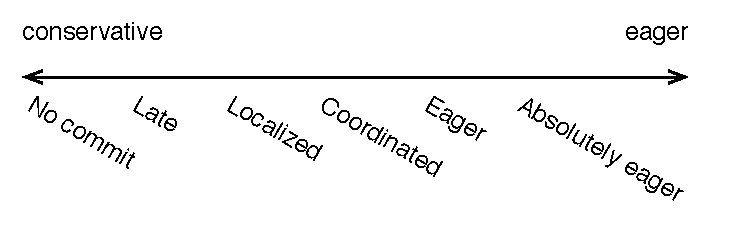
\includegraphics[width=0.4\textwidth]{commit-spectrum}
  \caption{Approximate Spectrum of Commit Semantics}
  \label{fig:commit-spectrum}
\end{figure}

Commits are used to control the run-time behavior,
mostly to prune choices for the purpose of performance.
The commit semantics described in Section \ref{sec:rules} and
in \figref{fig:rules} is called {\em localized commit} as it restricts
the scope of pruning to be of height 1 only.  $\cm$ by agent $X$ cannot
prune until the direct parent of the committed world is $\oplus_X$.
$\cu$ kills the current world immediately without coordination with other worlds.

Besides localized commit, in this section, we identify a number of other possible commit
semantics. They differ in their eagerness to prune the worlds.
They are ordered roughly from the most eager to the most conservative:
{\em absolutely eager commit}, {\em eager commit}, {\em coordinated commit}, {\em late commit}
and {\em no commit} (See \figref{fig:commit-spectrum}).
%The semantics of commits may be different and there are also 4 other commit semantics in order to support different types of pruning.
%They are the absolutely eager commit, the eager commit, the late commit, and the coordinated commit.
%Different commit semantics vary between the range of being conservative and eager, which is depicted in Figure \ref{fig:commit-spectrum}, where the ``none'' means no commit at all (i.e. to generate all the combinatorial choices).
%
We compare and contrast the behavior of these commit semantics
using the dining philosopher example and reason why localized commit
is the chosen semantics in the calculus.
Here we are only concerned with the shape of the tree structures
after different commits and ignore the details in the world (leaf nodes).
The initial structure is in \figref{fig:cmcmp:init},
and let's see the effect of $B$ committing in $w_1$.
\begin{description}
  \item[Absolutely eager commit] is the most aggressive form of commit and
as soon as one agent commits in one of the worlds,
it kills {\em all} the other worlds. As illustrated in
\figref{fig:cmcmp:abs}, system immediately prunes the whole sub-tree.

  \item[Eager commit] is less aggressive and kills the branch on the right
immediately once there is a commit in the branch on the left.
\footnote{Note that the terms ``left branch'' and ``right branch'' in this
discussion are symbolic and can be used interchangeably.}
This can be seen in \figref{fig:cmcmp:eager}.

  \item[Late commit] kills the branch on the right only if all occurrences
(not necessarily in the same scope) of the (syntactically) left branch commit.
In the example, it requires $B$ commits not only in $w_1$,
but also in $w_2$, $w_5$ and $w_7$ and prunes all the right-hand side of
$\oplus_B$ (\figref{fig:cmcmp:late}).

  \item[Coordinated commit] proposed in our previous work \cite{JaffarYZ07}
is a compromise between the eager commit and the late commit, which does not
kill the alternative choice until $\cm$ of this choice has been reached in
\emph{all} worlds in the {\em scope} of the choice construct.
In our example, this requires $B$ commits in both $w_1$ and $w_2$ and prunes
in the same way as the eager commit (\figref{fig:cmcmp:coord}).
%(i.e. the conjunctive view $\mathcal{CV}$); $\cu$ also uses $\mathcal{CV}$

  \item[No commit] is the naive behavior of ignoring all the $\cm$ or $\cu$
in the program. The net effect of this is that the universe can only grow and
doesn't shrink by itself even if all agents have reached completion and exit in all worlds.
The advantage of this is that if there is a solution for all the agents, this semantics
will find it, the disadvantage is the computation space is exponential.
If no-commit semantics is used, in this example, the shape of the tree
remains the same as the initial structure till the end.
To reclaim system resources, system could employ a global collapse rule below
to reduce a galaxy that has no more agents to a single world. And due to the
exit semantics and Property \ref{prop-exit},
any world in this galaxy can become the new galaxy.
\[
    \tag{\sc Collapse}\label{rule:collapse}
    \frac
    {\langle [], d, s \rangle \in leaves(G) }
    {G \gto \langle [], d, s \rangle}
\]


\item[Localized commit] cannot prune until $C$ commits in $w_1$ as well, because the reason for $B$ to commit in $w_1$ may be that $C$ lives in $w_1$. When $C$ commits in $w_1$, the tree structure becomes an intermediate state as shown in the left-hand side of Figure \ref{fig:cmcmp:local}. Then the pending commit from $B$ is executed and prunes in the same way as the absolutely eager commit eventually (right-hand side of Figure \ref{fig:cmcmp:local}). It is more conservative but can kill as many as the absolutely eager commit.
\end{description}

\begin{figure*}
\centering\small
\subfigure[Initial galaxy structure]{\label{fig:cmcmp:init}
\begin{minipage}{0.325\textwidth}
\Tree[.$\oplus_A$
    [.$\oplus_{B_1}$
        [.$\oplus_{C_1}$
            $w_1$
            $w_2$
        ]
        [.$\oplus_{C_2}$
            $w_3$
            $w_4$
        ]
    ]
    [.$\oplus_{C_3}$
        [.$\oplus_{B_2}$
            $w_5$
            $w_6$
        ]
        [.$\oplus_{B_3}$
            $w_7$
            $w_8$
        ]
    ]
]
\end{minipage}
}
\subfigure[Absolutely eager commit]{\label{fig:cmcmp:abs}
\begin{minipage}{0.195\textwidth}
\Tree[.$\oplus_A$
    $w_1$
    [.$\oplus_{C_3}$
        [.$\oplus_{B_2}$
            $w_5$
            $w_6$
        ]
        [.$\oplus_{B_3}$
            $w_7$
            $w_8$
        ]
    ]
]
\end{minipage}
}
\subfigure[Eager commit]{\label{fig:cmcmp:eager}
\begin{minipage}{0.225\textwidth}
\Tree[.$\oplus_A$
    [.$\oplus_{C_1}$
        $w_1$
        $w_2$
    ]
    [.$\oplus_{C_3}$
        [.$\oplus_{B_2}$
            $w_5$
            $w_6$
        ]
        [.$\oplus_{B_3}$
            $w_7$
            $w_8$
        ]
    ]
]
\end{minipage}
}
\subfigure[Late commit]{\label{fig:cmcmp:late}
\begin{minipage}{0.21\textwidth}
\centering
\begin{tabular}{c}
\\
\Tree[.$\oplus_A$
    [.$\oplus_{C_1}$
        $w_1$
        $w_2$
    ]
    [.$\oplus_{C_3}$
        $w_5$
        $w_7$
    ]
] \\ \\ \\
\end{tabular}
\end{minipage}
}
\subfigure[Coordinated commit]{\label{fig:cmcmp:coord}
\begin{minipage}{0.25\textwidth}
\Tree[.$\oplus_A$
    [.$\oplus_{C_1}$
        $w_1$
        $w_2$
    ]
    [.$\oplus_{C_3}$
        [.$\oplus_{B_2}$
            $w_5$
            $w_6$
        ]
        [.$\oplus_{B_3}$
            $w_7$
            $w_8$
        ]
    ]
]
\end{minipage}
}
\subfigure[Localized commit]{\label{fig:cmcmp:local}
\begin{tabular}{cccc}
$\quad$
&
\begin{minipage}{0.27\textwidth}
\Tree[.$\oplus_A$
    [.$\oplus_{B_1}$
        $w_1$
        [.$\oplus_{C_2}$
            $w_3$
            $w_4$
        ]
    ]
    [.$\oplus_{C_3}$
        [.$\oplus_{B_2}$
            $w_5$
            $w_6$
        ]
        [.$\oplus_{B_3}$
            $w_7$
            $w_8$
        ]
    ]
]
\end{minipage}
&
$\Rightarrow$
&
\begin{minipage}{0.18\textwidth}
\Tree[.$\oplus_A$
    $w_1$
    [.$\oplus_{C_3}$
        [.$\oplus_{B_2}$
            $w_5$
            $w_6$
        ]
        [.$\oplus_{B_3}$
            $w_7$
            $w_8$
        ]
    ]
]
\end{minipage}
\end{tabular}
}
\caption{Illustration of Different Commit Semantics}
\label{fig:cmcmp}
\end{figure*}

In general, the coordinated commit proposed previously \cite{JaffarYZ07}
has two disadvantages:
\begin{enumerate}
  \item The most attractive feature of coordinated commit is the ability to
  prune not only leaf worlds but also subtrees of worlds,
  but the condition for this to happen requires $\cm$ of this choice to be reached
  in the scope of the choice construct, in all worlds.
  However, it is costly to do so as it needs to maintain information
	of the {\em conjunctive views} of many data stores. \footnote{Conjunctive view
of a set of stores $D$ is the common data in $D$.}
  \item As shown in the following example, it may prune the only world
	where all agents can be satisfied.
\end{enumerate}

\begin{figure}[th]
  \centering
  \small\Tree[.$\oplus_X$
          [.$\oplus_Y$
            {$X:+\alpha.\cm_1$\\$Y:\underline{-\beta}.\cm$\\ \\ $(X_l Y_l)$}
            {$X:+\alpha.\cm_2$\\$Y:\underline{-\gamma}.\cm$\\ \\ $(X_l Y_r)$}
          ]
          [.$\oplus_Y$
            {$X:+\beta.\cm_3$\\$Y:-\beta.\cm_5$\\ \\$(X_r Y_l)$}
            {$X:+\beta.\cm_4$\\$Y:\underline{-\gamma}.\cm$\\ \\ $(X_r Y_r)$}
          ]
        ]
  \caption{Runtime Galaxy Structure for Programs $X$ and $Y$}
  \label{fig:commit-example}
\end{figure}


Let's consider the following simple program to understand why the localized commit is better
than the other pruning-based commit semantics and chosen as the default semantics in
our calculus. Suppose there are two agent programs $X$ and $Y$:
\begin{eqnarray*}
  X: & +\alpha.\cm\oplus +\beta.\cm \\
  Y: & -\beta.\cm\oplus -\gamma.\cm
\end{eqnarray*}

A possible runtime galaxy structure is shown in Figure \ref{fig:commit-example}
where $\oplus_X$ starts before $\oplus_Y$.
$X$ and $Y$ are subscripted with $l$ and $r$ which means
the left-hand side and the right-hand side respectively.
The underlined parts are blocked while all other operations can be executed successfully.
Subscripts of $\cm$ indicate the execution order of the commit actions.
Consider the effects of different commit semantics in Figure \ref{fig:commit-example}.

Absolutely eager commit prunes all the three worlds $X_l Y_r$, $X_r Y_l$ and $X_r Y_r$
when $\cm_1$ is executed.
Eager commit prunes both $X_r Y_l$ and $X_r Y_r$ when $\cm_1$ is executed.
Late commit waits until both $\cm_1$ and $\cm_2$ are executed and then prunes both
$X_r Y_l$ and $X_r Y_r$.
Coordinated commit is the same as late commit in this example.
Localized commit prevents $\cm_1$ and $\cm_2$ from pruning worlds
because the commits are issued by $X$ while the parent of $X_l Y_l$ and $X_l Y_r$ is $Y$;
only until $\cm_5$ is executed in world $X_r Y_l$ and
prunes $X_r Y_r$, the pending commit $\cm_3$ prunes both
$X_l Y_l$ and $X_l Y_r$.

\section{Analysis}

We present preliminary statistical findings from ShibaScript, including lexical analysis and transcribing accuracy evaluation.
% \KZ{rewrite this preamble, it's irrelevant now: To give a detailed picture about our dataset ShibaScript and also show several statistical syntax results on it, we will explain our analysis below.}

% This is the analysis on this dataset. Inlcuding its distribution and some further analysis inlcuding bigrams.

% \subsection{Source Information}
% \label{sec:sourceinformation}
% The 16 dogs come from 16 different Japanese user accounts at YouTube. From the videos uploaded from the specific user and the captions attached to these videos, we can get to know much about the growing up environments of dogs, which will influence the expressions of these dogs to some degree. %The environments of them are in \ref{tab:sourceinformation}.
%这是狗的来源的信息,包含地区、是否家养、之类的

% \begin{table}[th]
% \centering
% \begin{tabular}{c|c|c|c}
% \hline
% \textbf{Dog Index} & \textbf{Color} & \textbf{Other Pets} & \textbf{Area}\\\hline
% 0 & yellow & \\
% 1 & yellow & \\
% 2 & yellow & \\
% 3 & yellow & \\
% 4 & yellow & \\
% 5 & yellow & \\
% 6 & yellow & \\
% 7 & yellow & \\
% 8 & yellow & \\
% 9 & yellow & True \\
% 10 & yellow & \\
% 11 & yellow & \\
% 12 & yellow & \\
% 13 & yellow & \\
% 14 & yellow & \\
% 15 & black & \\\hline
% \end{tabular}
% \caption{The source information of dogs in ShibaScript. Color means the fur color of the dog. Other Pets means whether the dog is kept with a family with other animals. Area means the living locations of the family.}
% \label{tab:sourceinformation}
% \end{table}



% \begin{table}
% \centering
% \begin{tabular}{c|c|c|c|c}
% \hline
% \multirow{2}{*}{\textbf{DogID}} & \multicolumn{2}{c|}{\textbf{Sentence}} & \multicolumn{2}{c}{\textbf{Word}}  \\
% \cline{2-5}
% {} & \textbf{Num} & \textbf{Length(s)} & \textbf{Num} & \textbf{Length(s)} \\
% \cline{1-5}
% 0 & 346 & 1107.67 & 577 & 363.36\\
% 1 &  158 & 514.24 & 241 & 129.00\\
% 2 & 553 & 1643.00 & 847 & 469.20\\
% 3 &  55 & 171.69 & 123 & 65.52\\
% 4 & 56 & 224.00 & 107 & 94.08\\
% 5 &  115 & 374.58 & 217 & 98.52\\
% 6 & 52 & 157.00 & 77 & 47.72\\
% 7 & 40 & 135.00 & 65 & 27.44\\
% 8 &  135 & 566.03 & 316 & 143.68\\
% 9 & 255 & 795.00 & 408 & 157.08\\
% 10 & 1188 & 4306.00 & 2029 & 1372.52\\
% 11& 188 & 570.94 & 320 & 203.20\\
% 12  & 130 & 562.28 & 257 & 147.00\\
% 13  & 993 & 2930.19 & 1719 & 749.72\\
% 14  & 118 & 350.11 & 324 & 144.76\\
% 15  & 87 & 299.88 & 134 & 101.24 \\\hline
% sum & \textbf{4469} & \textbf{14707.61} & 7761 & 4314.04\\\hline
% \end{tabular}
% \caption{The basic statistical information of ShibaScript.}
% \label{tab:datasetinformation}
% \end{table}




\subsection{Lexical Analysis}
During the transcribing, there are in total 11 types of tokens, in which 9 types are phonetic symbols~(\tabref{tab:alphabet}), the other two are short pauses between words and long pauses between sentences. 

Similar to humans, the length of these tokens contain ample information. The exact lengths of tokens are kept in ShibaScript for concrete analysis. Because the long pauses are largely determined by the scene at that time, the numerical analysis of it will not be included here. 


\begin{table}[th]
\centering
\small
\begin{tabular}{c|c|c}
\hline
\textbf{Symbol} & \textbf{Mean len (s)} & \textbf{Variance (s)}\\
\hline
\verb|[au]| & 0.35 & 0.022 \\
\verb|[a]| & 0.35 & 0.017 \\
\verb|[^]| & 0.34 & 0.017\\
\verb|[u:]| & 0.45 & 0.054\\
\verb|[u]| & 0.35 & 0.030\\
\verb|[i]| & 0.33 & 0.020\\
\verb|[k]| &  0.24 & 0.009\\
\verb|[(w)au]| & 0.34 & 0.018\\
\verb|[en]| & 0.36 & 0.032\\
\verb|short pause| & 0.57 & 0.335\\
\hline
\end{tabular}
\caption{The mean and variance of the duration of 9 phonetic symbols 
and short pauses between words.}
\label{tab:tokenanalysis}
\end{table}

The mean and variance of each token length can be seen in~\tabref{tab:tokenanalysis}. In which we find that almost every phonetic symbol has a similar length of 0.35s or so. Except for the phonetic symbol \verb|[u:]|, which is a prolonged sound owning an average length of 0.45s. While phonetic symbol \verb|[k]| is a relatively short-lived symbol, only having 0.24s average length.

Considering the monogram~(\figref{fig:monogram}) of ShibaScript, we can find that the most frequent symbol is \verb|[en]|, which reaches to 3478 times in ShibaScript, the following two are \verb|[au]| and \verb|[a]|, which reaches  1981 and 2011 times respectively. One of the reasons why \verb|[en]| exceeds much, which is counterintuitive, is that symbols such as \verb|[a]|, \verb|[au]|, \verb|[(w)au]| are divided up. The least frequent symbol is \verb|[k]|, which only reaches 15 times. This is because dogs seldom produce air-sounds like \verb|[k]|.

At the same time, we can find that these phonetic symbols exist in multiple dogs' sounds, showing that these 9 symbols are universal.

\begin{figure}[th]
\centering
\scalebox{0.32}{\includegraphics{monogram.pdf}}
\caption{The occurrences of each monogram. The blue bars show the occurrences across the whole dataset of each monogram in ShibaScript, the green lines show the numbers of dogs producing the symbols, from 1 to 16.}%\KZ{Remove ``Monogram Stats'' from the pic, since
% you already talk about it in the caption.}
\label{fig:monogram}
\end{figure}

%静音片段分析
%unigram, bigram分析
After analyzing the monogram, we come to find the relationship between symbols, as well as the bigram~(\figref{fig:bigram}) of ShibaScript. Among these bigrams, several appear extremely frequently. It shows a possibility that they are associated with some common semantic meanings. We will dive into that in the future works. Due to space constraints, the detailed information of bigram is shown in~\secref{sec:appendixc}.

% 1 
\begin{figure}[th]
\centering
\scalebox{0.32}{\includegraphics{bigram.pdf}}
\caption{The occurrences of each bigram. The blue bars show the occurrences across the whole dataset of each monogram in ShibaScript, the green lines show the numbers of dogs producing the symbols, from 1 to 16.}
\label{fig:bigram}
\end{figure}




\subsection{Accuracy of Transcription}
In this paper, we discover the certain phonetic pattern of Shiba Inu dogs and assign a vocal dictionary of 9 symbols, which is a first-step trial in this area. To better evaluate the phonetic symbols set as well as the integral accuracy of our transcribing, we have done an evaluation test on these two aspects. The evaluation metric is 5-level Mean Opinion Score~\cite{viswanathan2005measuring}. Three raters will give scores to either one syllable or one word according to~\tabref{tab:ratestandard}. %\MY{How many raters?}


\begin{table}[th]
\centering
\small
\begin{tabular}{c|l}
\hline
\textbf{Score} & \textbf{Description} \\
\hline
5 & The label exactly matches up.\\
4 & Some difference exists between the\\
{}& label and the sound. Humans are s- \\
  & ometimes hard to distinguish.\\
3 & Difference exists between the label\\
  & and the sound. Humans can tell the \\
  & difference immediately.\\
2 & Although the label is obviously wr-\\
{}& ong, there is similarity between t-\\
{}& he label and the sound.\\
1 & The label is totally wrong. \\
% 5 - Excellent 完全一致,失真程度不可察觉
% 4 - Good 有轻微不一致,失真程度略可察觉,如a和ao, u和u:,(w)au 和au,人耳有时也会难以分辨其中差异
% 3 - Fair 一般,失真程度可察觉,人耳可以轻松分辨出二者差异
% 2 - Poor 差,失真程度尚可接受,可以找到一丝相似
% 1 - Bad 很差,失真程度难以接受, 完全不同
\hline
\end{tabular}
\caption{The evaluation metric of rating, which is similar to MOS in speech synthesis evaluation metric.}
\label{tab:ratestandard}
\end{table}

\subsubsection{Phonetic Symbol Accuracy Evaluation}
\label{sec:phone_eva}
%在音素层面进行的evaluation
For each syllable category, we select 50 syllables randomly. The rating result is in~\figref{fig:phoneticaccuracy}. The Fleiss Kappa~\cite{kilicc2015kappa} between three annotators is 0.609.

\begin{figure}[th]
\centering
\scalebox{0.30}{\includegraphics{phoneticaccuracy.pdf}}
\caption{The evaluation result of 9 phonetic symbols. }
\label{fig:phoneticaccuracy}
\end{figure}

% \KZ{Fonts too small, and the image is not clear. Every image must be critical clear after ampification. Use vector images (not bitmap) whenever possible.}

\subsubsection{Word Accuracy Evaluation}
%在word层面进行的evaluation
For the word accuracy evaluation, we select 30 words for each dog randomly and find the same person who rates for phonetic symbols to score for them. The rating result is in~\figref{fig:wordaccuracy}. The Fleiss Kappa between three annotators is 0.516.

\begin{figure}[th]
\centering
\scalebox{0.29}{\includegraphics{wordaccuracy.pdf}}
\caption{The evaluation result of words for 16 different dogs.}
\label{fig:wordaccuracy}
\end{figure}

